\section{Метрики классификации} 

Ошибки классификации бывают \textbf{False Positive} и \textbf{False Negative}. В статистике первый вид ошибок называют ошибкой I-го рода, а второй — ошибкой II-го рода.

\begin{center}
    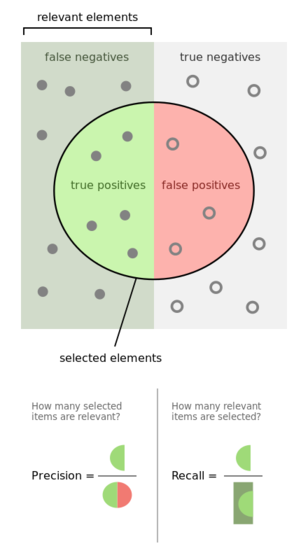
\includegraphics[scale=0.8]{tickets/pictures/diag.png}
\end{center}

\subsection{Accuracy}
$$
\text { accuracy }=\frac{T P+T N}{T P+T N+F P+F N}
$$

\textbf{Accuracy} - это доля правильных ответов алгоритма. Эта метрика бесполезна в задачах с неравными классами.

\subsection{Precision}
$$
\text { precision }=\frac{T P}{T P+F P}
$$

\textbf{Precision} - это доля объектов, названных классификатором положительными и при этом действительно являющимися положительными.

\subsection{Recall}
$$
\text { recall }=\frac{T P}{T P+F N}
$$

\textbf{Recall} - это доля объектов положительного класса из всех объектов положительного класса.

\textit{Recall} демонстрирует способность алгоритма обнаруживать данный класс вообще, а \textit{precision} — способность отличать этот класс от других классов.

\subsection{F - мера}
$$
F_{\beta}=\left(1+\beta^{2}\right) \cdot \frac{\text { precision } \cdot \text { recall }}{\left(\beta^{2} \cdot \text { precision }\right)+\text { recall }}
$$

\textbf{F-мера} (в общем случае $F_{\beta}$) — среднее гармоническое \textit{precision} и \textit{recall}.

$\beta$ в данном случае определяет вес точности в метрике, и при $\beta=1$ это среднее гармоническое (с множителем 2, чтобы в случае \textit{precision} = 1 и \textit{recall} = 1 иметь $F_{1}=1$).

\textbf{F-мера} достигает максимума при полноте и точности, равными единице, и близка к нулю, если один из аргументов близок к нулю (гармоническое среднее, в отличие от арифметического, стремится к нулю, когда хотя бы одно из значений стремится к нулю).

\subsection{ROC-AUC}

\textbf{ROC AUC} — площадь (Area Under Curve) под кривой ошибок (Receiver Operating Characteristic curve ). Данная кривая представляет из себя линию от (0,0) до (1,1) в координатах \textit{True Positive Rate (TPR)} и \textit{False Positive Rate (FPR)}:

$$
\begin{aligned}
T P R &=\frac{T P}{T P+F N} \\
F P R &=\frac{F P}{F P+T N}
\end{aligned}
$$
\begin{center}
    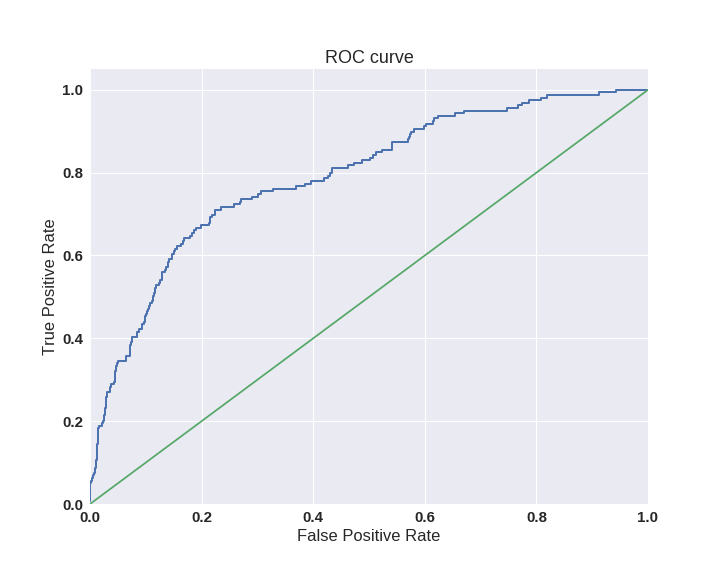
\includegraphics[scale=0.6]{tickets/pictures/curve.png}
\end{center}

\subsection{LogLoss}
$$
\text { logloss }=-\frac{1}{l} \cdot \sum_{i=1}^{l}\left(y_{i} \cdot \log \left(\hat{y}_{i}\right)+\left(1-y_{i}\right) \cdot \log \left(1-\hat{y}_{i}\right)\right)
$$

Здесь $\hat{y}$ - это ответ алгоритма на $i$ -ом объекте, $y-$ истинная метка класса на $i$ -ом объекте, а $l$ размер
выборки.

Можно представить минимизацию \textit{logloss} как задачу максимизации \textit{accuracy} путем штрафа за неверные предсказания. Однако \textit{logloss} крайне сильно штрафует за уверенность классификатора в неверном ответе.

\subsection{Мультиклассовые задачи}

Основные подходы сведения мультиклассовой задачи к бинарным: \textbf{one-vs-all} (K бинарных классификаторов для каждого класса против всего остального) и \textbf{all-vs-all} ($C_{K}^{2}$ классификаторов для попарно различных классов, результат - класс с наибольшим количеством голосов).

Выделяют два подхода сведения подсчета качества к метрикам классификации: \textbf{микро-} и \textbf{макро-усреднение}.

Пусть выборка состоит из $K$ классов. Рассмотрим $K$ двухклассовых задач, каждая из которых заключается в отделении своего класса от остальных, для них можно вычислить $\mathrm{TP}_{k}, \mathrm{FP}_{k}, \mathrm{FN}_{k}, \mathrm{TN}_{k} .$
\subsection*{Микро-усреднение}
При \textit{микро-усреднении} сначала эти характеристики усредняются по всем классам, а затем вычисляется итоговая двухклассовая метрика - например, \textit{точность}, \textit{полнота} или \textit{F-мера}. Например, \textit{точность} будет вычисляться по формуле
$$
\operatorname{precision}(a, X)=\frac{\overline{\mathrm{TP}}}{\overline{\mathrm{TP}}+\overline{\mathrm{FP}}}
$$
где, например, $\overline{\mathrm{TP}}$ вычисляется по формуле
$$
\overline{\mathrm{TP}}=\frac{1}{K} \sum_{k=1}^{K} \mathrm{TP}_{k}
$$
\subsection*{Макро-усреднение}
При \textit{макро-усреднении} сначала вычисляется итоговая метрика для каждого класса, а затем результаты усредняются по всем классам. Например, \textit{точность} будет
вычислена как
$$
\operatorname{precision}(a, X)=\frac{1}{K} \sum_{k=1}^{K} \operatorname{precision}_{k}(a, X) ; \quad \text { precision }_{k}(a, X)=\frac{\mathrm{TP}_{k}}{\mathrm{TP}_{k}+\mathrm{FP}_{k}}
$$